\chapter{Hipótesis de estudio}\label{sec:chapterVII}
\addcontentsline{toc}{chapter}{Hipótesis de estudio}

A pesar de que el estudio descriptivo anterior muestra unos datos muy variados, casi todos ellos son homogéneos año tras año. Es decir, todos los años son diferentes pero las variables recogidas año tras año presentan la misma distribución de probabilidad. No obstante, el objetivo de este estudio es sentar las bases para conseguir una experiencia de aprendizaje óptima para todos los grupos de alumnos. Así pues, se va a poner énfasis en detectar a aquellos grupos que estén en riesgo de obtener un peor rendimiento o peores calificaciones. La detección temprana de éstos podría permitir al profesorado actuar a tiempo para mejorar su proceso de aprendizaje. Para ello, se van a proponer una serie de métricas de calidad que se definirán sobre los registros de actividad de los alumnos con el objetivo de encontrar aquella que, con mayor certeza, identifique a los alumnos que peor están progresando.

\section{Métricas de calidad y correlaciones entre ellas}

Se definirán dos grandes grupos de métricas. El primer grupo consistirá en una colección de métricas de los grupos que solamente podrán calcularse tras la finalización de la práctica. Por el contrario, las métricas del segundo grupo podrán calcularse durante la realización de la práctica y, por tanto, serán más interesantes porque podrán facilitar la detección precoz de los grupos en riesgo.

Gráficamente, las medidas clásicas del rendimiento del estudiantado se han representado en la Figura \ref{fig:measures}.

\begin{figure}[H]
    \centering
    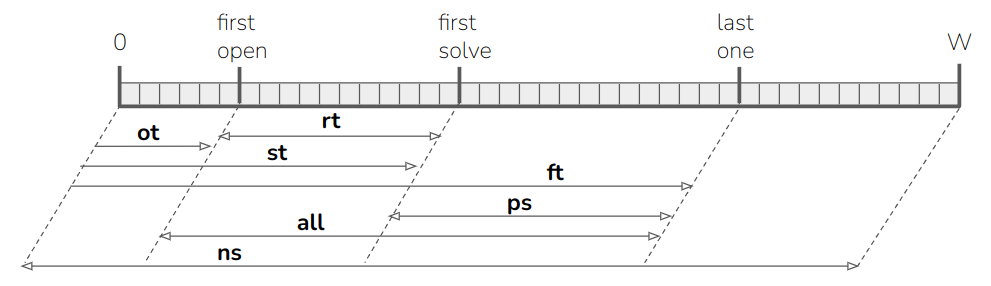
\includegraphics[width=\textwidth]{hipótesis/measures.png}
    \caption{Representación gráfica de las medidas de rendimiento empleadas que se extraen directamente de los registros del servidor (no se incluyen las medidas derivadas del análisis espectral de grafos).}
    \label{fig:measures}
\end{figure}

\subsection{Medidas a posteriori del resultado de la práctica}

\begin{itemize}
\item La calificación conseguida por el alumno (\emph{Grade}). Obviamente, cuanto mayor sea ésta, mejor.
\item Número de problemas resueltos u objetivos resueltos. Se denotará por \emph{p}. Trivialmente, cuantos más objetivos haya resuelto un grupo, mejor. El número de problemas normalizado se denotará por \emph{np} en los estudios que se realizarán a continuación.
\item Punto de finalización de toda la práctica. En la Figura \ref{fig:measures}  se representa esta medida de rendimiento normalizada (dado que la duración de la práctica no es la misma todos los años) por \emph{ft}. Cuanto antes, mejor (para disponer de más tiempo para repasar y corregir errores). Sin embargo, no es una métrica muy relevante.
\item Tiempo consumido por el alumno durante las prácticas. Éste es un valor trampa, pues puede significar algo positivo (el alumno ha tardado poco en resolver la práctica porque la domina), o negativo (porque no ha podido dedicarle más tiempo). En la Figura \ref{fig:measures}, el tiempo consumido normalizado se representa por \emph{all}.
\item Número de sesiones realizadas (\emph{s}). Ya se ha hecho un estudio de esta medida en la sección \ref{sec:activityrecorded}. En la Figura \ref{fig:measures}, se representa el número de sesiones normalizado (\emph{ns}).
\end{itemize}

\subsection{Medidas continuas durante la práctica}

\begin{itemize}
\item Como los comienzos son siempre costosos, se definirá una nueva métrica correspondiente al promedio de tiempo de la primera apertura de cada problema. Se representa por \emph{ot} en la Figura \ref{fig:measures}.
\item Número de fails consecutivos (\emph{fail ratio} o \emph{fr}) hasta resolver un problema dividido entre el número de sesiones de ese problema. La tasa de fallo así como el tiempo dedicado a un mismo problema dependerá de la dificultad del mismo.
%\item \emph{También se definirá una medida que cuantificará la posposición de tareas de los grupos. Es decir, pretende identificar a aquellos alumnos que, cuando intentan resolver un problema y no lo consiguen, saltan, curiosamente, a otros problemas más complejos (los cuales, obviamente, tampoco pueden resolver) perdiendo así un tiempo precioso.}
\item Tiempo promedio empleado en resolver los problemas (representado por \emph{rt}).
\item Tiempo promedio empleado en los problemas tras su resolución. Se representa por \emph{ps} en la Figura \ref{fig:measures} y trata de evidenciar el interés de los alumnos en la materia. En general, será positivo que los grupos no sólo resuelvan los problemas sino que traten de encontrar mejores soluciones para los mismos como se podrá ver en el Capítulo \ref{chapter:correlations}.
\item Tiempo promedio de resolución de los problemas por primera vez. Se representará por \emph{st} en la Figura \ref{fig:measures}.
\item Se tendrá igualmente una medida que refleja si los grupos de prácticas siguen el orden esperado de las mismas. Se le denotará por \emph{sq} en los análisis que se realizarán posteriormente.
\item Todas las medidas de complejidad definidas en la Sección \ref{sec:complexity}.
\end{itemize}